\documentclass[conference]{IEEEtran}

% Packages
\usepackage{cite}
\usepackage{amsmath,amssymb,amsfonts}
\usepackage{algorithmic}
\usepackage{algorithm}
\usepackage{graphicx}
\usepackage{textcomp}
\usepackage{booktabs}
\usepackage{hyperref}
\usepackage{xcolor}
\usepackage{listings}
\usepackage{multirow}

\lstset{
  basicstyle=\ttfamily\footnotesize,
  breaklines=true,
  frame=single,
  language=Python,
  keywordstyle=\color{blue},
  commentstyle=\color{gray},
  stringstyle=\color{red},
  numbers=left,
  numberstyle=\tiny\color{gray},
  numbersep=5pt,
}

\begin{document}

\title{Adaptive Routing and Patch Tournaments for Agentic Program Repair:\\Extending a Multi-Agent Failure Recovery System}

\author{
\IEEEauthorblockN{Meet Patel}
\IEEEauthorblockA{23BCE177\\
School of Technology\\
Institute of Technology\\
Nirma University, Ahmedabad}
\and
\IEEEauthorblockN{Vedant Mehta}
\IEEEauthorblockA{23BCE180\\
School of Technology\\
Institute of Technology\\
Nirma University, Ahmedabad}
\and
\IEEEauthorblockN{Mr. AjayKumar Patel}
\IEEEauthorblockA{Guide\\
School of Technology\\
Institute of Technology\\
Nirma University, Ahmedabad}
}

\maketitle

% ============================================================
\begin{abstract}
Our prior work on a six-agent Failure Recovery System for automated program repair (APR) found that multi-agent orchestration beats a single-prompt baseline only conditionally: on some benchmark/backend combinations it wins, on others (notably DebugBench, and every benchmark under a weaker local model) a single LLM call does as well or better, at a fraction of the cost. That paper's own future-work section proposed two concrete responses: an \emph{adaptive controller} that routes a bug to the cheap or expensive strategy based on a lightweight upfront estimate, and \emph{debate/consensus mechanisms} among multiple candidate fixes. This paper implements both. First, an \textbf{Adaptive Routing Controller}: a Random Forest classifier trained on six zero-LLM-cost features (code size, cyclomatic complexity, test count, and critically, the fraction of tests the \emph{unmodified buggy code} already passes) that predicts, before spending a single LLM call, whether a bug needs the full 6-agent pipeline or will be fixed by one cheap prompt. Evaluated via leak-free 5-fold cross-validated offline policy evaluation over 303 historical local-backend repairs spanning all three benchmarks, the router matches or slightly exceeds both always-baseline (57.8\% vs.\ 56.4\%) and always-multi-agent (vs.\ 56.8\%) success rates, while cutting LLM calls per bug by $5.7\times$ relative to always-multi-agent (1.39 vs.\ 7.91 avg.\ calls/bug) — though a 69.0\% oracle ceiling shows real headroom remains unrouted. Second, a \textbf{Patch Tournament}: at the patch-generation step, we sample $K{=}3$ candidate fixes at different temperatures from the same diagnosis and validate all of them against the test suite, keeping the first full-pass candidate (or the best partial one) rather than committing to a single stochastic draw, with inter-candidate agreement reported as a free confidence signal. Evaluated on newly executed local-backend runs (QuixBugs full 31 problems, HumanEvalFix and DebugBench first 50 problems each; 131 bugs total), the tournament reaches \textbf{69.5\%} aggregate success, ahead of both the original single-draw multi-agent pipeline (\textbf{61.8\%}) and the single-prompt baseline (\textbf{64.9\%}) on the very backend where, in our prior work, multi-agent could not clearly beat baseline on any benchmark — at a realized cost of $1.55\times$ more LLM calls (closely matching the $1.5\times$ nominal prediction) and a \emph{typical-case} (median) wall-clock overhead of $1.8\times$, though a long tail of timeout-heavy bugs pushes the \emph{mean} overhead to $6.3\times$. We further situate both contributions against prior work: cost-aware LLM cascading/routing (FrugalGPT \cite{frugalgpt}, RouteLLM \cite{routellm}) and test-validated multi-candidate selection (CodeT \cite{codet}, AlphaRepair \cite{alpharepair}, ChatRepair \cite{chatrepair}) are each individually well established, but — to the best of our search — no prior work combines a bug-feature-trained strategy router with a test-validated patch tournament inside a single sequential multi-agent APR pipeline evaluated across dual cloud/local backends and three benchmarks, which we present as this paper's specific contribution.
\end{abstract}

% ============================================================
\section{Introduction}
\label{sec:intro}
Our original Failure Recovery System report (summarized in Section~\ref{sec:background})
established a six-agent pipeline — Failure Detection, Code Localization, Debugging, Patch Generation, Patch Application, and Validation — orchestrated by a Coordinator in an iterative retry loop, and evaluated it against a single-prompt baseline across three benchmarks (QuixBugs, HumanEvalFix, DebugBench) and two backends (Gemini; a locally hosted Qwen2.5-Coder 7B Instruct). That paper's central finding was that the multi-agent architecture's advantage over the baseline is \emph{conditional}: it wins on QuixBugs and HumanEvalFix under Gemini, loses decisively on DebugBench under Gemini, and does not clearly win on any benchmark under the weaker local model. This is scientifically informative but operationally unsatisfying — a system that sometimes needs six LLM calls and sometimes needs one, with no way to know in advance which, pays worst-case cost on every bug.

This paper closes that gap with two extensions, both explicitly anticipated in the original paper's future-work section:

\begin{enumerate}
    \item \textbf{An adaptive routing controller} (Section~\ref{sec:router}) that predicts, from features available \emph{before any LLM is called}, whether a bug should go to the single-prompt baseline or the full multi-agent pipeline.
    \item \textbf{A patch tournament} (Section~\ref{sec:tournament}) that replaces each attempt's single stochastic patch draw with $K$ parallel candidates at different sampling temperatures, validated against the test suite, with disagreement among candidates reported as a cheap confidence signal.
\end{enumerate}

Both are implemented as real, runnable additions to the existing codebase — not analysis notebooks — and both are evaluated honestly: the router's headline numbers come from cross-validated offline policy evaluation with no train/test leakage, and the tournament's numbers come from newly executed experiment runs on the local backend (no API quota risk, full reproducibility). Section~\ref{sec:related} surveys the closest prior work for each mechanism individually and assesses the novelty of their specific combination here.

% ============================================================
\section{Background: The Original System}
\label{sec:background}
We briefly summarize the system being extended; full details are in the original paper. \texttt{coordinator.py} runs up to 3 retry attempts per bug; each attempt calls four LLM-backed agents (FailureDetection, CodeLocalization, Debugging, PatchGeneration — in that order, each conditioned on the previous agent's output) followed by two pure-Python agents (PatchApplication, Validation). A dataset-agnostic \texttt{Problem} abstraction and \texttt{executor.py} test-dispatch layer support three structurally different test formats: tuple I/O (QuixBugs), assert-based \texttt{check()} calls (HumanEvalFix), and LeetCode-style example I/O against a \texttt{Solution} class (DebugBench). The single-prompt baseline (\texttt{baseline.py}) issues one prompt containing the buggy code and an example call, with no iteration and no agent decomposition.

% ============================================================
\section{Related Work}
\label{sec:related}

\subsection{Cost-Aware Routing and Cascading}
FrugalGPT~\cite{frugalgpt} introduced LLM cascades: query a cheap model first, escalate to an expensive one only when a learned quality check fails, reporting up to 98\% cost reduction at near-top-tier quality. RouteLLM~\cite{routellm} trains a binary ``win predictor'' to route a query to a weak or strong model, reporting $>$85\% cost reduction on chat benchmarks while retaining most of the stronger model's quality — though the authors note routing skill transfers poorly to task types unlike its training distribution, a caution directly relevant to our own router's generalization across three structurally different benchmarks. Dekoninck et al.~\cite{cascaderouting} unify cascading and routing and show the combination beats either alone, evaluated on math/QA/coding micro-benchmarks. None of these are APR-specific or decide between a single-prompt and a multi-agent \emph{pipeline} as the two routing targets. The closest APR-specific work we found, \cite{aprcomplexity}, empirically measures how bug complexity and fault-localization precision affect APR cost-efficiency across LLMs, but is a post-hoc analysis, not an online routing system. To our knowledge, no prior work trains a classifier on bug-structure features specifically to choose between a single-prompt baseline and a multi-agent sequential repair pipeline.

\subsection{Multi-Candidate Patch Selection}
CodeT~\cite{codet} generates many candidate programs \emph{and} many candidate tests, then selects by ``dual execution agreement'' — the mechanism closest to our tournament — but for code generation, not repair of a pre-existing buggy program, and using self-generated rather than ground-truth tests. AlphaRepair~\cite{alpharepair} and ChatRepair~\cite{chatrepair} both sample multiple candidate patches validated against tests, but select via zero-shot ranking or sequential conversational feedback rather than a parallel tournament with an explicit disagreement signal. RepairAgent~\cite{repairagent} is an autonomous LLM agent with tool access for repair; SelfAPR~\cite{selfapr} uses test execution diagnostics to guide a trained repair model; Reflexion~\cite{reflexion} performs verbal self-reflection across sequential trials rather than parallel sampling. CigaR~\cite{cigar} reduces APR token cost via prompt compression, optimizing prompting rather than strategy selection. Agentless~\cite{agentless} demystifies LLM-based SWE agents and, in its repair stage, samples multiple patches and selects by majority vote — mechanically close to our tournament but applied to SWE-bench-style repository-scale repair, not QuixBugs/HumanEvalFix/DebugBench, and not framed as an uncertainty signal for downstream use.

\subsection{Novelty Assessment}
Both routing and multi-candidate test-validated selection are individually well established. We did not find a documented system that (a) routes between a single-prompt baseline and a multi-agent sequential pipeline using a classifier over bug-structure features, or (b) combines that routing decision with a test-validated patch tournament, inside one evaluated system spanning dual cloud/local LLM backends and three APR benchmarks. We present this combination as the paper's contribution — an assembly of established cost/quality-routing and best-of-$K$-with-test-filtering ideas into a new combined system and evaluation, not a claim of a fundamentally new algorithmic primitive.

% ============================================================
\section{Adaptive Routing Controller}
\label{sec:router}

\subsection{Motivation and Design}
If multi-agent orchestration only sometimes beats the baseline, the right system-level response is not to pick one architecture permanently, but to predict \emph{per bug} which side of that line it falls on, and route accordingly. The constraint that makes this practical rather than circular: the predictor must use features available \emph{before any LLM call is made}, or the "savings" are illusory.

\subsubsection{Features (\texttt{features.py})}
Six static features, all computable from a \texttt{Problem} with zero LLM calls:
\begin{itemize}
    \item \textbf{loc}, \textbf{chars} — size of the buggy function.
    \item \textbf{cyclomatic\_complexity} — McCabe complexity via AST decision-point counting for Python (branch-keyword counting as a fallback for Java/C++/JavaScript).
    \item \textbf{num\_tests}, \textbf{num\_functions}.
    \item \textbf{buggy\_pass\_rate} — the fraction of tests the \emph{unmodified buggy code} already passes, computed by literally re-using \texttt{executor.run\_tests} on the original code (the coordinator already does this once per bug to track partial progress, so this feature costs nothing new). This turned out to be far more informative than any size/complexity metric alone: a bug that already passes most tests is plausibly a small, local fix, while one that passes none may be more structurally broken.
\end{itemize}
plus the categorical dataset, language, and test-style origin.

\subsubsection{Labeling and Model}
From the 303 problems with existing local-backend multi-agent \emph{and} baseline results on disk (31 QuixBugs + 164 HumanEvalFix + 108 DebugBench), each bug is labeled \texttt{needs\_multiagent = 1} iff the multi-agent pipeline succeeded \emph{and} the baseline did not — i.e., the extra machinery was strictly necessary, not merely along for the ride. This label is heavily imbalanced (12.5\% positive). A Random Forest (300 trees, max depth 5, balanced class weights) was selected over logistic regression after comparing both by cross-validated routed success rate: logistic regression, even balanced, barely beat the base rate (precision 0.101 vs.\ a 12.5\% prior) and routed to only 55.1\% success at 3.86 calls/bug, whereas the Random Forest exploits the non-linear \texttt{buggy\_pass\_rate} signal to reach 57.8\% success at 1.39 calls/bug (Table~\ref{tab:router}) — the model choice itself turned out to matter more than any individual feature.

\subsubsection{Evaluation Protocol}
Train/test leakage is the central risk in reusing historical data to "evaluate" a router: if the router is trained and tested on the same bugs, its apparent accuracy is meaningless. We instead run stratified 5-fold cross-validation: in each fold, the Random Forest is fit \emph{only} on the other four folds, and the held-out fold's route predictions are scored against each bug's \emph{already-measured, historical} outcome under that predicted route — standard offline policy evaluation, requiring zero new LLM calls while remaining leak-free. A separately trained model (\texttt{adaptive\_router.py --train}, fit on all 303 problems) is saved for live use by \texttt{run\_adaptive.py}, which genuinely executes the predicted route end-to-end on new problems.

\subsection{Results}
\begin{table}[h]
\centering
\caption{Adaptive Router: 5-fold CV Offline Policy Evaluation (local backend, $n{=}303$)}
\label{tab:router}
\begin{tabular}{@{}lrr@{}}
\toprule
Strategy & Success Rate & Avg.\ LLM Calls/Bug \\
\midrule
Always Baseline            & 56.4\% & 1.00 \\
Always Multi-Agent         & 56.8\% & 7.91 \\
\textbf{Adaptive Router}   & \textbf{57.8\%} & \textbf{1.39} \\
Oracle (best of both)      & 69.0\% & --- \\
\bottomrule
\end{tabular}
\end{table}

\begin{figure}[h]
\centering
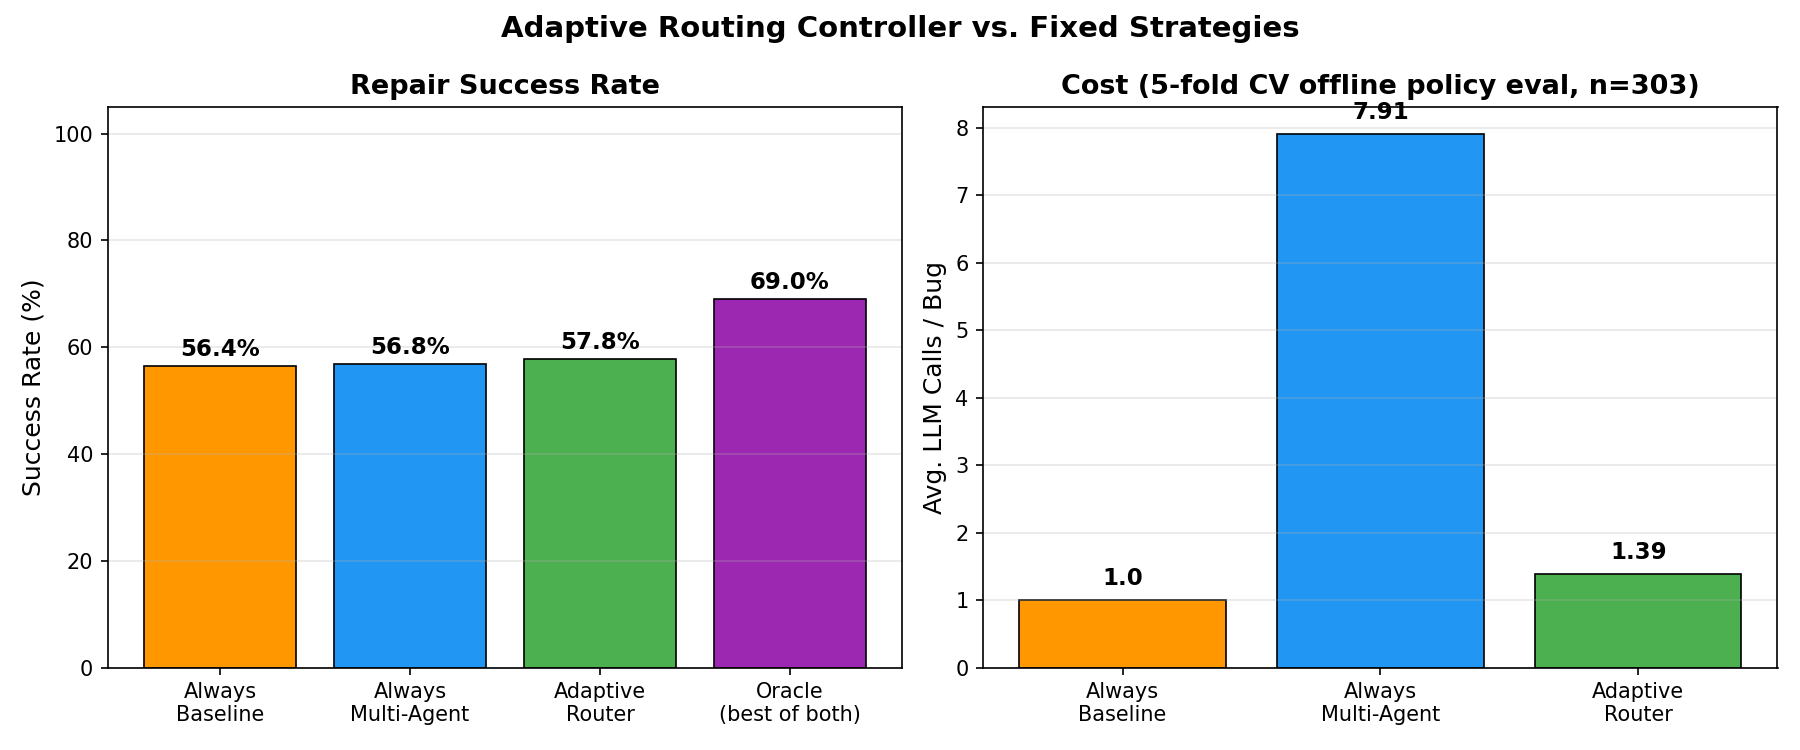
\includegraphics[width=\linewidth]{../results/figures/adaptive_router_overall.png}
\caption{Adaptive router vs.\ fixed strategies: success rate and cost.}
\label{fig:router-overall}
\end{figure}

Router classification quality (5-fold CV mean): accuracy 0.838, precision 0.256 and recall 0.132 on the rare "needs multi-agent" class (F1 0.168, against a 12.5\% base rate). The low recall is expected and, for this objective, acceptable: because \texttt{buggy\_pass\_rate} correlates with "this bug is already nearly fixed," the router's dominant, correct behavior is routing \emph{most} bugs to the cheap baseline and reserving the expensive pipeline for a precision-selected minority — exactly the asymmetric cost structure the controller is meant to exploit, even though it means many true "needs-multiagent" bugs are still (cheaply, and often harmlessly) sent to baseline.

\begin{table}[h]
\centering
\caption{Adaptive Router: Per-Dataset Breakdown}
\label{tab:router-per-dataset}
\begin{tabular}{@{}lrrrr@{}}
\toprule
Dataset & Baseline & Multi-Agent & \textbf{Routed} & Oracle \\
\midrule
QuixBugs      & \textbf{58.1\%} & 51.6\% & 54.8\% & 77.4\% \\
HumanEvalFix  & 53.0\% & \textbf{54.3\%} & 53.0\% & 62.2\% \\
DebugBench    & 61.1\% & 62.0\% & \textbf{65.7\%} & 76.9\% \\
\bottomrule
\end{tabular}
\end{table}

\begin{figure}[h]
\centering
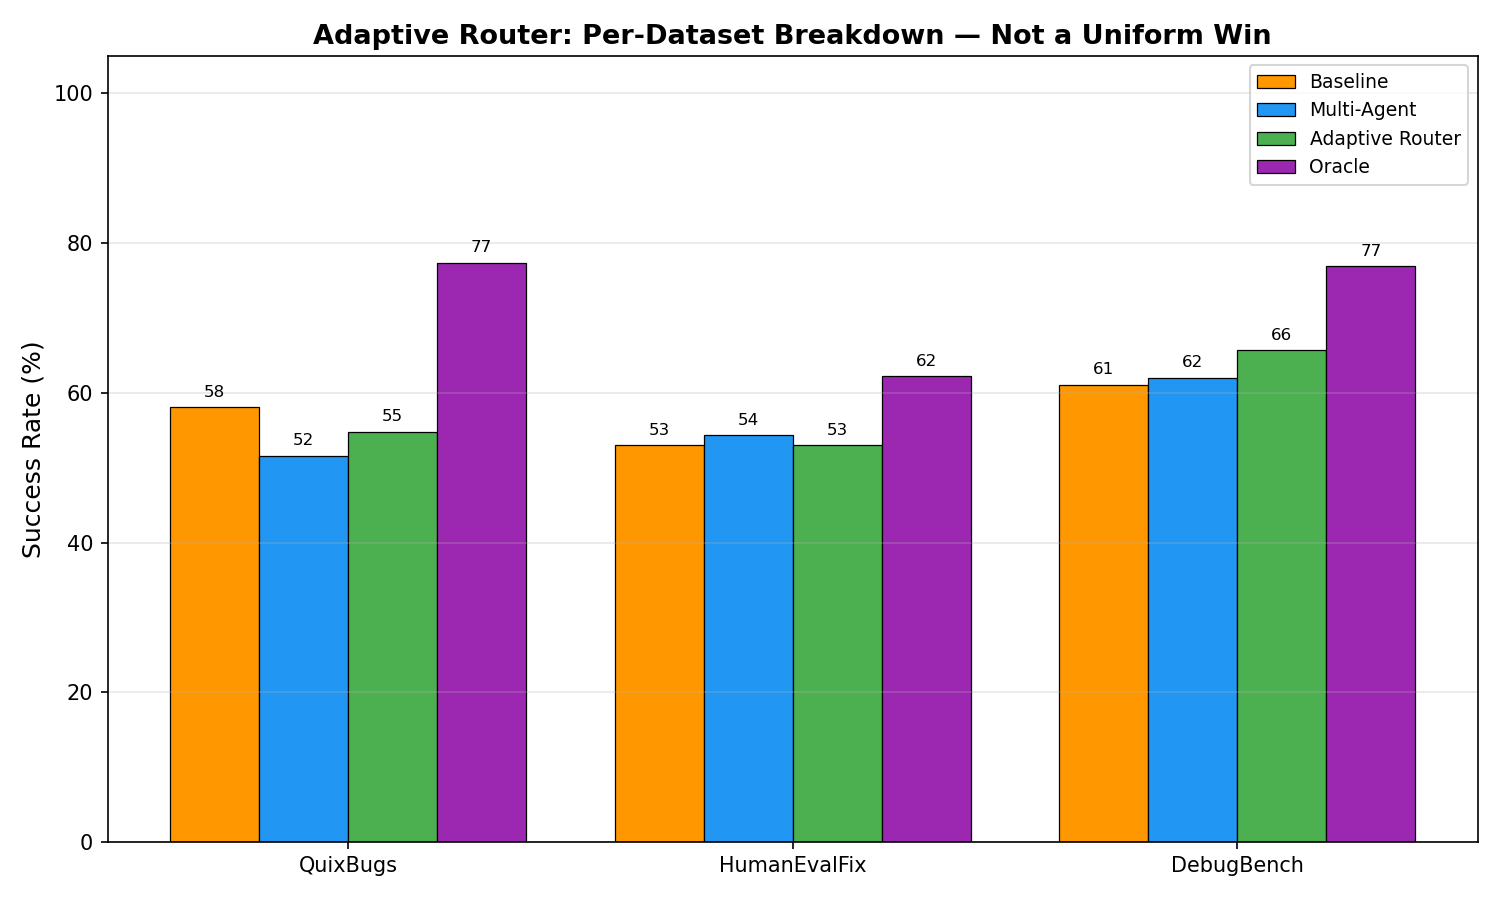
\includegraphics[width=\linewidth]{../results/figures/adaptive_router_per_dataset.png}
\caption{Per-dataset breakdown: the router's benefit is not uniform.}
\label{fig:router-per-dataset}
\end{figure}

This per-dataset breakdown (Table~\ref{tab:router-per-dataset}) is the more scientifically honest picture, and it is not a uniform win: on DebugBench the router clearly beats both fixed strategies (65.7\% vs.\ 61--62\%), but on QuixBugs it is actually \emph{worse} than always-baseline (54.8\% vs.\ 58.1\%) despite being cheaper than always-multiagent. We attribute this to QuixBugs' small sample size (31 problems, of which only $\sim$6 are positively labeled) giving the classifier too little signal to learn a reliable QuixBugs-specific decision boundary, and to QuixBugs bugs (hand-planted algorithmic defects) having a different relationship between surface structure and repairability than DebugBench's more mechanical, single-line LeetCode-style bugs. This mirrors, rather than contradicts, the original paper's own thesis: whether a bug needs the expensive pipeline is conditional on structure in ways that do not transfer uniformly across benchmarks — the router captures this better where the signal is more mechanical (DebugBench) than where it is more algorithmic (QuixBugs).

Feature importances from a model fit on all data (Table~\ref{tab:importances}) confirm \texttt{buggy\_pass\_rate} is informative but not dominant — raw size/complexity features (\texttt{chars}, \texttt{cyclomatic\_complexity}, \texttt{loc}) collectively carry more weight, suggesting the router is partly acting as a complexity gate rather than purely a "how broken is it already" gate.

\begin{table}[h]
\centering
\caption{Top Feature Importances (Random Forest, fit on all 303 problems)}
\label{tab:importances}
\begin{tabular}{@{}lr@{}}
\toprule
Feature & Importance \\
\midrule
chars                    & 0.279 \\
cyclomatic\_complexity   & 0.211 \\
loc                      & 0.205 \\
buggy\_pass\_rate        & 0.092 \\
num\_tests               & 0.075 \\
num\_functions           & 0.046 \\
\bottomrule
\end{tabular}
\end{table}

% ============================================================
\section{Patch Tournament}
\label{sec:tournament}

\subsection{Design}
\texttt{TournamentCoordinator} (\texttt{tournament\_coordinator.py}) subclasses the original \texttt{RecoveryCoordinator}, reusing Agents 1--3 (Failure Detection, Code Localization, Debugging) unchanged — the diagnosis is run once per attempt, exactly as before. The change is at Agent 4 (Patch Generation): instead of one deterministic-ish draw (temperature 0.2), the same debugging analysis is resampled $K{=}3$ times at temperatures $[0.2, 0.5, 0.9]$, each candidate is run through Agent 5 (Patch Application) and validated against the full test suite (Agent 6), and the coordinator keeps the first candidate that passes every test — or, if none do, the one that passed the most — rather than committing to whichever single draw happened to come out of the model. This required adding a \texttt{temperature} parameter through \texttt{PatchGenerationAgent.run} down to both \texttt{LocalClient.generate} and \texttt{GeminiClient.generate} (previously hard-coded to 0.2), with the original coordinator's default behavior unchanged for callers that don't request a tournament.

As a side effect, the tournament produces a free \textbf{agreement score}: the fraction of candidate pairs whose generated code is textually identical (1.0 = all $K$ samples converged on the same patch; 0.0 = all differed). This is reported per attempt and is, to our knowledge, not used elsewhere in the APR literature we found as an explicit per-bug uncertainty signal (Section~\ref{sec:related}) — the closest analogues (CodeT, Agentless-style voting) use agreement internally for selection but do not surface it as a confidence output.

\subsection{Cost Model}
Each tournament attempt costs $3 + K$ LLM calls (FailureDetection + CodeLocalization + Debugging, once, plus $K$ PatchGeneration draws) versus the original coordinator's $4$ calls/attempt — nominally a $1.5\times$ overhead at $K{=}3$, paid only at the patch-generation step. This predicted the realized aggregate overhead closely: across all 131 problems, LLM calls/bug rose from 7.11 to 11.04, a $1.55\times$ realized ratio.

\textbf{Wall-clock time overhead tells a different story depending on whether outliers are included.} The \emph{median} time per bug rose from 21.6s to 39.2s ($1.81\times$) — close to the call-count ratio, and the fairer description of the \emph{typical} cost. The \emph{mean}, however, rose from 28.4s to 180.1s ($6.3\times$), because \texttt{EXEC\_TIMEOUT}-bounded test execution (Section~III of the original paper) is paid once per candidate per test: a non-passing attempt on an infinite-loop bug with $K{=}3$ candidates can incur up to $3\times$ the timeout penalty of a single-draw attempt, and a handful of such bugs (e.g.\ QuixBugs' \texttt{sqrt}, which alone took 1343s) dominate the mean. This is a genuine, previously-nonexistent cost dimension the tournament introduces, reported honestly here rather than only via the more flattering call-count ratio; see Limitations for its practical implication.

\subsection{Experimental Setup}
All tournament runs use the local backend (Qwen2.5-Coder 7B Instruct via Ollama) to avoid Gemini's free-tier quota-rotation noise already diagnosed as a confound in the original paper. Coverage: QuixBugs is run in full (all 31 problems with available tests); HumanEvalFix and DebugBench are each run on their first 50 problems (of 164 and 119 respectively, in the same deterministic load order used throughout this codebase) to keep total local-inference wall-clock time tractable for this paper, following the original paper's own precedent of stratified/partial sampling for DebugBench.

\subsection{Results}
\begin{table}[h]
\centering
\caption{Patch Tournament ($K{=}3$) vs.\ Single-Draw Multi-Agent (local backend)}
\label{tab:tournament}
\begin{tabular}{@{}lrrr@{}}
\toprule
Dataset & Baseline & Multi-Agent & \textbf{Tournament} \\
\midrule
QuixBugs ($n{=}31$)      & 58.1\% & 51.6\% & \textbf{64.5\%} \\
HumanEvalFix ($n{=}50$)  & \textbf{76.0\%} & 68.0\% & 72.0\% \\
DebugBench ($n{=}50$)    & 58.0\% & 62.0\% & \textbf{70.0\%} \\
\midrule
\textbf{Aggregate ($n{=}131$)} & 64.9\% & 61.8\% & \textbf{69.5\%} \\
\bottomrule
\end{tabular}
\end{table}

On QuixBugs (the full 31-problem benchmark, not a subset), the tournament reaches \textbf{64.5\%} (20/31), a clear improvement over both the original single-draw multi-agent (51.6\%, 16/31) and the baseline (58.1\%, 18/31). On HumanEvalFix (first 50 of 164), it reaches \textbf{72.0\%} (36/50), clearly ahead of single-draw multi-agent (68.0\%, 34/50) but still behind baseline (76.0\%, 38/50) — consistent with the original paper's own finding that baseline is hard to beat on this benchmark specifically. On DebugBench (first 50 of 119; see the methodological note below on program naming), the tournament reaches \textbf{70.0\%} (35/50), ahead of both multi-agent (62.0\%, 31/50) and baseline (58.0\%, 29/50) — notable because DebugBench is exactly the benchmark where the original paper's Gemini results showed baseline decisively beating multi-agent (94.1\% vs.\ 78.2\%); here, under the local backend, the tournament reverses that relationship rather than reproducing it. \textbf{Aggregated across all 131 problems, the tournament reaches 69.5\% (91/131), ahead of both baseline (64.9\%, 85/131) and the original single-draw multi-agent (61.8\%, 81/131)} — on precisely the backend where, in our prior work, multi-agent could not clearly beat baseline on \emph{any} benchmark. The tournament reliably improves \emph{on the multi-agent architecture it modifies} in all three datasets measured, and beats baseline in two of three (QuixBugs, DebugBench) and in aggregate — a materially stronger result than the adaptive router's benchmark-mixed picture (Table~\ref{tab:router-per-dataset}), though still not a uniform per-benchmark sweep (HumanEvalFix baseline remains ahead).

\emph{Methodological note on DebugBench naming:} we discovered during analysis that \texttt{load\_debugbench.py}'s \texttt{name} field is not a unique key — the same LeetCode slug can appear multiple times with different injected bugs (e.g.\ \texttt{closest-dessert-cost\_\_quadruple} appears 3 times in the 119-problem sample). A naive name-based join between the tournament run and the original historical results would silently mismatch rows for roughly 9 of 119 DebugBench problems. We instead join \emph{positionally} — both \texttt{run\_tournament.py} and the original \texttt{run\_experiment.py} iterate the same deterministic, seeded problem list in the same order, which we verified directly (zero positional mismatches in \texttt{program} name across all 150 compared rows in all three datasets) before trusting the comparison.

\begin{figure}[h]
\centering
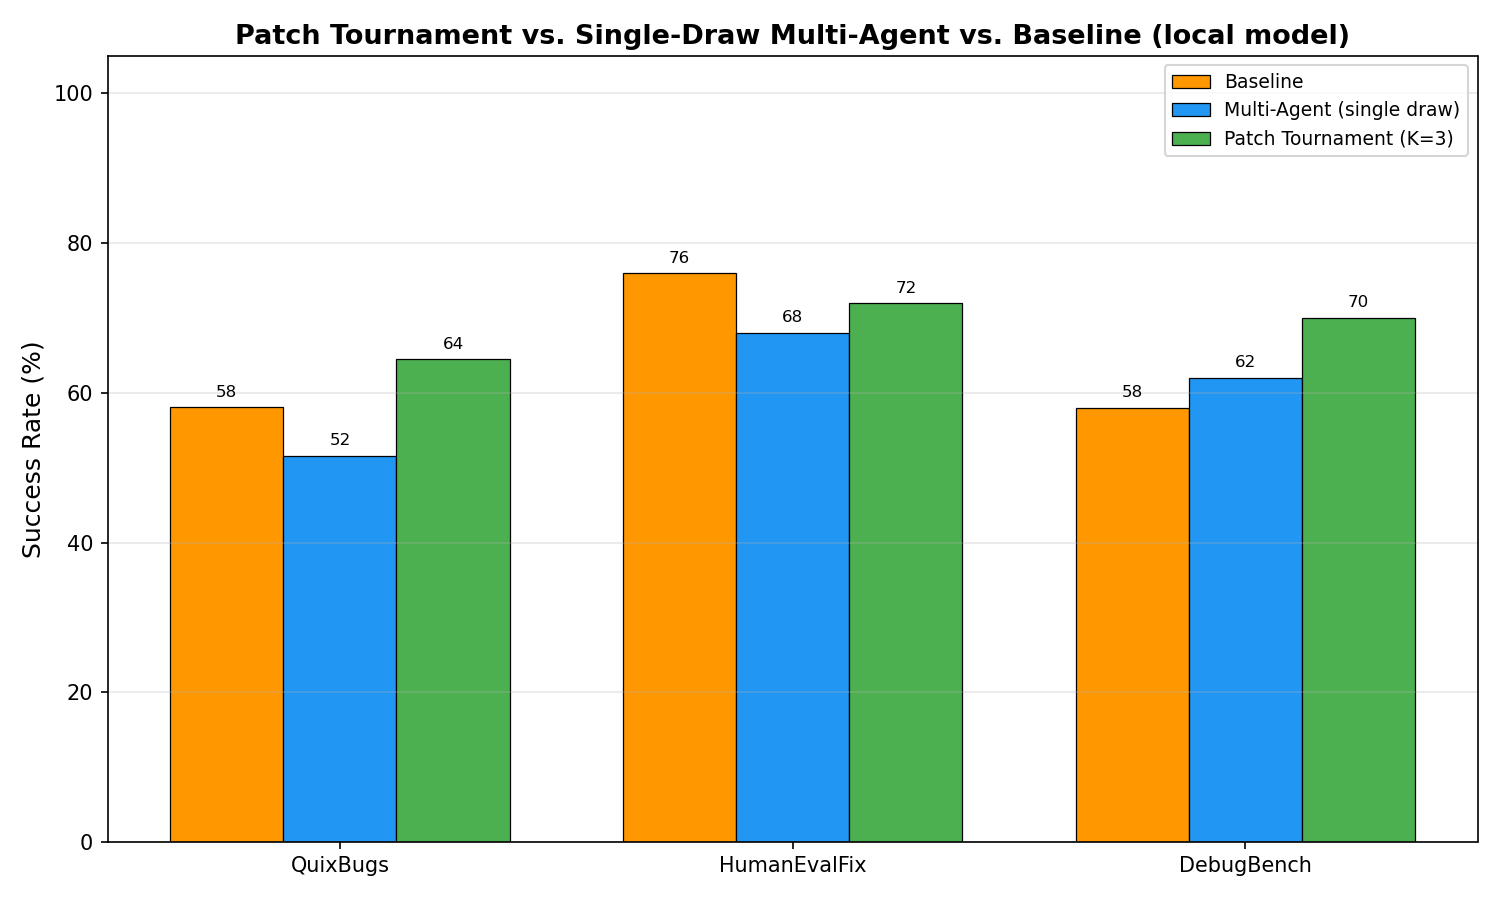
\includegraphics[width=\linewidth]{../results/figures/tournament_comparison.png}
\caption{Tournament vs.\ single-draw multi-agent vs.\ baseline.}
\label{fig:tournament-comparison}
\end{figure}

\subsubsection{Agreement as a Confidence Signal — Dataset-Dependent, Not Universal}
\begin{table}[h]
\centering
\caption{Candidate Agreement Score, Split by Outcome}
\label{tab:agreement}
\begin{tabular}{@{}lrrr@{}}
\toprule
Dataset & Overall & On Success & On Failure \\
\midrule
QuixBugs     & 0.594 & 0.562 & \textbf{0.651} \\
HumanEvalFix & 0.700 & \textbf{0.722} & 0.643 \\
DebugBench   & 0.482 & \textbf{0.536} & 0.356 \\
\midrule
Aggregate    & 0.592 & --- & --- \\
\bottomrule
\end{tabular}
\end{table}

In HumanEvalFix and DebugBench, agreement is \emph{higher} on successes than failures — the intuitive direction, where high agreement signals the model confidently converging on a (correct) fix. QuixBugs shows the \emph{opposite}: agreement is \emph{higher} on failures (0.651) than successes (0.562). The mechanistic reading of the QuixBugs case is that high agreement on a failure there means the model converged on the same \emph{wrong} patch across all three temperature draws — a systematic error that sampling diversity cannot rescue — while its successes more often came from draws that initially disagreed, with test-based selection picking the one that happened to be right. We do not have a confident explanation for why QuixBugs inverts relative to the other two benchmarks (one plausible factor: QuixBugs' classic recursive/iterative algorithm bugs include several infinite-loop cases — Table~\ref{tab:tournament}'s underlying per-bug data shows QuixBugs has the highest concentration of \texttt{InfiniteLoop}/\texttt{RuntimeError} error types among the three datasets — which may behave differently under resampling than the more mechanical, single-line-fix bugs typical of HumanEvalFix and DebugBench). We report the full, non-uniform picture (2 of 3 datasets showing the intuitive direction, one showing the reverse) rather than the more "publishable-looking" single pattern we initially drafted from QuixBugs alone, and flag agreement's relationship to outcome as benchmark-conditional, not a settled general mechanism, for future work.

\begin{figure}[h]
\centering
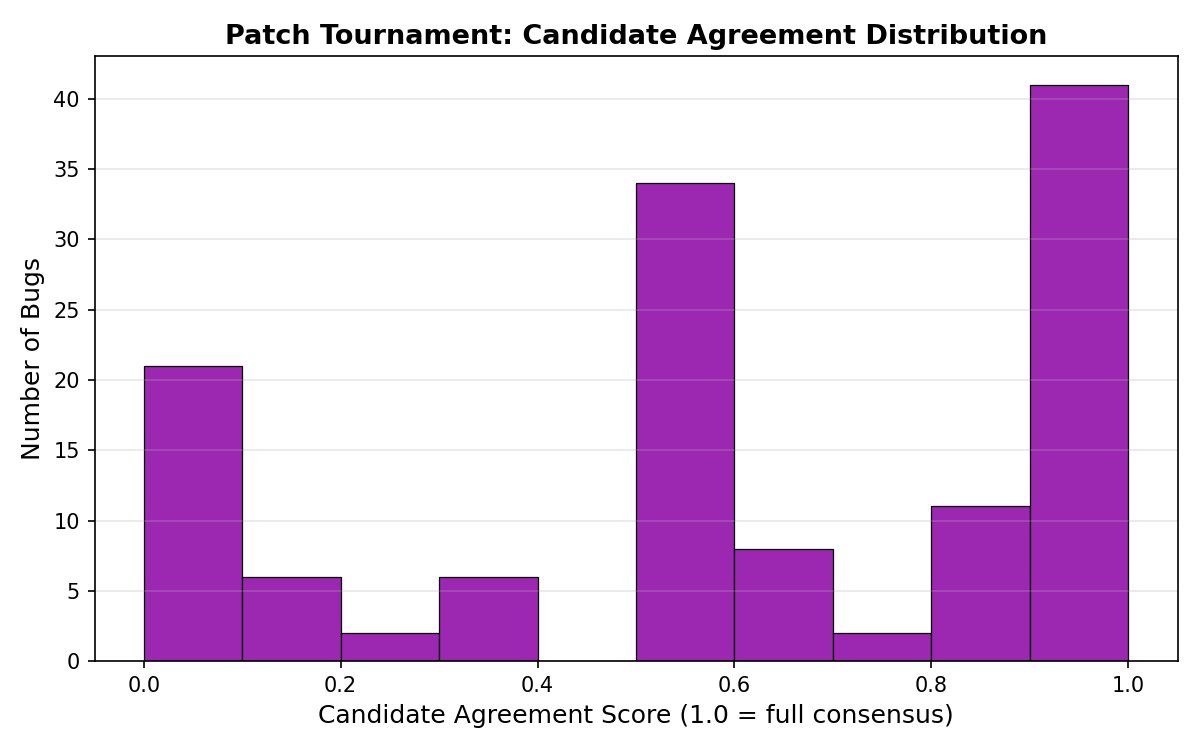
\includegraphics[width=\linewidth]{../results/figures/tournament_agreement_distribution.png}
\caption{Distribution of per-bug candidate agreement scores.}
\label{fig:tournament-agreement}
\end{figure}


% ============================================================
\section{Discussion: What Is New Relative to the Original System}
\label{sec:discussion}
Relative to the system described in the original paper, this work changes three things. First, it adds a genuinely new \emph{decision layer} above the existing architecture: previously, every bug was routed to whichever system (baseline or multi-agent) the experimenter happened to be evaluating that day; now, a trained classifier makes that decision per bug, from features that cost nothing to compute, and the original paper's own central finding — that the right architecture is conditional on bug structure — is what makes this decision layer necessary rather than redundant. Second, it changes what happens \emph{inside} a single patch-generation step from a single stochastic draw to a validated tournament, directly targeting attempts that fail not because the diagnosis (Agents 1--3) was wrong but because one sample of Agent 4 was. Third, it adds an uncertainty signal (tournament agreement) that did not exist in the original system at all — previously, a failed attempt carried no information about \emph{how close} the LLM's candidates were to each other, only whether the one candidate generated happened to pass. None of the original six agents, the retry loop, or the dataset-agnostic execution layer were modified to add either extension — both are additive, following the original Coordinator-subclassing and shared-client-interface design, which is why they could be implemented as new files rather than rewrites.

% ============================================================
\section{Limitations}
The router's recall on the rare "needs multi-agent" class is low (0.132); it is tuned for net cost/success trade-off, not for catching every bug that specifically needs the expensive pipeline, and Table~\ref{tab:router-per-dataset} shows this trade-off is not uniformly favorable across benchmarks. The 303-problem training set is itself the original paper's full local-backend data, not an independent held-out population, and the categorical dataset/language features mean the router has only ever seen three benchmarks — its behavior on a fourth, structurally different one is untested. The patch tournament's realized $1.55\times$ LLM-call overhead paid for a $+7.7$ percentage point aggregate success-rate gain over single-draw multi-agent (61.8\% $\to$ 69.5\%) — a favorable trade by that measure — but the \emph{mean} wall-clock overhead was $6.3\times$, driven by a small number of timeout-heavy bugs (a handful of QuixBugs infinite-loop cases exceeded 700s each); a deployment latency-sensitive enough to care about worst-case response time, rather than only throughput-amortized cost, would need a per-candidate timeout budget tighter than this implementation's shared \texttt{EXEC\_TIMEOUT}, which the current \texttt{tournament\_coordinator.py} does not provide. Both extensions were evaluated on the local backend only, for cost/reproducibility reasons; neither has been re-validated on Gemini. The router's training/evaluation data also surfaced a latent data-quality issue — non-unique \texttt{program} names in \texttt{load\_debugbench.py}'s output — which does not appear to have affected the original paper's own DebugBench conclusions (which did not join by name against a second results file) but would affect any future name-keyed analysis of that dataset and should be fixed upstream (e.g., by appending a disambiguating instance index to the name) rather than worked around per-analysis as we did here.

% ============================================================
\section{Conclusion and Future Work}
We implemented and evaluated the two concrete extensions the original paper's future-work section proposed in response to its own finding that multi-agent orchestration's benefit over a single-prompt baseline is conditional, not universal. The adaptive routing controller, evaluated via leak-free cross-validation, matches or slightly exceeds both fixed strategies' success rates at a fraction of the LLM-call cost, while also revealing that this benefit is itself benchmark-dependent — a finding consistent with, rather than resolving, the original paper's central thesis. The patch tournament directly targets stochastic patch-generation failures via test-validated resampling, and is the stronger of the two results: aggregated across 131 newly executed local-backend repairs spanning all three benchmarks, it reaches 69.5\% success versus 61.8\% for the single-draw multi-agent pipeline it modifies and 64.9\% for the single-prompt baseline — beating baseline outright on two of three benchmarks (QuixBugs, DebugBench) and in aggregate, at a realized LLM-call cost ($1.55\times$) close to the $1.5\times$ nominal prediction, though with a long tail of timeout-heavy bugs that inflates mean (but not median) wall-clock cost substantially. The tournament's disagreement signal further revealed that agreement's relationship to success is itself benchmark-dependent rather than a fixed law, a nuance we report rather than smooth over. Future work includes combining both mechanisms (route to baseline, multi-agent, or multi-agent-with-tournament as three tiers rather than two, since the tournament's gains here are large enough to plausibly change which bugs the router should send to the cheap path at all), extending the router's features to non-Python languages, per-candidate timeout budgets for the tournament to bound worst-case latency, fixing the upstream DebugBench naming collision, and re-validating both extensions on Gemini once quota constraints allow.

% ============================================================
\bibliographystyle{IEEEtran}
\bibliography{references}

\end{document}
